%--------------------------------------------------------------------
% NE 155 (intro to numerical simulation of radiation transport)
% Spring 2017

% formatting
\documentclass[12pt]{article}
\usepackage[top=1in, bottom=1in, left=1in, right=1in]{geometry}

\usepackage{setspace}
\onehalfspacing

\setlength{\parindent}{0mm} \setlength{\parskip}{1em}


% packages
\usepackage{amssymb}
%% The amsthm package provides extended theorem environments
\usepackage{amsthm}
\usepackage{epsfig}
\usepackage{times}
\renewcommand{\ttdefault}{cmtt}
\usepackage{amsmath}
\usepackage{graphicx} % for graphics files

% Draw figures yourself
\usepackage{tikz} 

% The float package HAS to load before hyperref
\usepackage{float} % for psuedocode formatting
\usepackage{xspace}

% from Denovo methods manual
\usepackage{mathrsfs}
\usepackage[mathcal]{euscript}
\usepackage{color}
\usepackage{array}

\usepackage[pdftex]{hyperref}

\newcommand{\nth}{n\ensuremath{^{\text{th}}} }
\newcommand{\ve}[1]{\ensuremath{\mathbf{#1}}}
\newcommand{\macro}{\ensuremath{\Sigma}}
\newcommand{\vOmega}{\ensuremath{\hat{\Omega}}}

\newcommand{\cc}[1]{\ensuremath{\overline{#1}}}
\newcommand{\ccm}[1]{\ensuremath{\overline{\mathbf{#1}}}}


%--------------------------------------------------------------------
%--------------------------------------------------------------------
\begin{document}
\begin{center}
{\bf NE 155, Classes 16 \& 17, S17 \\
Iterative Solutions for Linear Systems \\ February 24 and 27, 2017}
\end{center}

\setlength{\unitlength}{1in}
\begin{picture}(6,.1) 
\put(0,0) {\line(1,0){6.25}}         
\end{picture}

%--------------------------------------------------------------------
\section*{Solutions of Linear Systems}

Recall: Given $\ve{A}\vec{x} = \vec{b}$, how do you find $\vec{x}$?

We talked about how to do this directly, now we'll talk about how to do this other ways.

\begin{itemize}  
\item Iterative Methods
  \begin{itemize}
  \item produce a sequence of vectors, $\vec{x}^{(1)}, \vec{x}^{(2)}, \dots$ based on the prescription
  \[\vec{x}^{(k+1)} = F(\vec{x}^{(k)}, \vec{b})\:, \qquad \text{where } \displaystyle \lim_{k \rightarrow \infty} \vec{x}^{(k)} = \vec{x}\]
  \item can require many FLOPs; storage requirements for $\ve	{A}$ can be an issue (if stored)
  \item may parallelize well
  \item \emph{often} used in practice
  \item used in smoothing methods and as pre-conditioners
  \item Jacobi, Gauss-Seidel, SOR, Multigrid, ...
  \end{itemize}
  
\item Semi-Iterative Methods
  \begin{itemize}
    \item produce a sequence of vectors, $\vec{x}^{(1)}, \vec{x}^{(2)}, \dots$ based on the prescription
  \[\vec{x}^{(k+1)} = F(\vec{x}^{(k)}, \vec{x}^{(k-1)}, \dots, \vec{x}^{(0)}, \vec{b})\:, \qquad \text{where } \displaystyle \lim_{k \rightarrow \infty} \vec{x}^{(k)} = \vec{x}\]  
  The function does not necessarily have to use all previous $\vec{x}$ iterates.
  \item can require many FLOPs; storage requirements for $\ve	{A}$ can be an issue (if stored)
  \item may parallelize well
  \item Commonly used in conjugate gradients, generalized minimal residuals methods
  \end{itemize}
\end{itemize}


%--------------------------------------------------------------------
%--------------------------------------------------------------------
\section*{Iterative Methods}
We need iterative methods when our system of linear equations is large. Recall: produce a sequence of vectors, $\vec{x}^{(1)}, \vec{x}^{(2)}, \dots$ based on the prescription
  \[\vec{x}^{(k+1)} = F(\vec{x}^{(k)}, \vec{b})\:, \qquad \text{where } \displaystyle \lim_{k \rightarrow \infty} \vec{x}^{(k)} = \vec{x}\] 

We will write this as \[\vec{x}^{(k+1)} = \ve{P}\vec{x}^{(k)} +  \tilde{\vec{b}}\:,\qquad k = 0, 1, \dots \]

We will add a matrix $\ve{S}$ to both sides to execute our process.
%
\begin{align}
(\ve{A} + \ve{S}) \vec{x} &= \ve{S}\vec{x} + \vec{b} \nonumber \\
%
\ve{Q} \vec{x} &= \ve{S}\vec{x} + \vec{b} 
\qquad\text{where } \ve{Q} = \ve{A} + \ve{S} \nonumber \\
%
\vec{x} &= \underbrace{\ve{Q}^{-1} \ve{S}}_{\ve{P}}\vec{x} + \underbrace{\ve{Q}^{-1} \vec{b}}_{\tilde{\vec{b}} }
\qquad\text{assuming regular } \ve{Q}\nonumber
\end{align}
%
The \textbf{fixed-point} iterative process is:
\begin{align}
\vec{x}^{(0)} &= \text{ arbitrary}\nonumber \\
\vec{x}^{(k+1)} &= \ve{P}\vec{x}^{(k)} + \tilde{\vec{b}} \nonumber
\end{align}

To determine convergence, we define the iterative error as follows, noting that $\vec{x}$ is defined as the solution to $\ve{A}\vec{x} = \vec{b}$. 
%
\begin{align}
\vec{e}^{(k)} &= \vec{x}^{(k)} - \vec{x} \nonumber \\
%
&\text{Subtract the exact solution from the method} \nonumber \\
%
\vec{x}^{(k+1)} &= \ve{P}\vec{x}^{(k)} + \tilde{\vec{b}} \nonumber \\
- (\vec{x} &= \ve{P}\vec{x} + \tilde{\vec{b}}) \nonumber \\
%
\vec{x}^{(k+1)} - \vec{x} &= \ve{P}(\vec{x}^{(k)} - \vec{x})\nonumber \\
%
\nonumber \\
%
\text{Thus, } \vec{e}^{(k+1)} &= \ve{P}\vec{e}^{(k)} \nonumber \\
%
\text{Further, } \vec{e}^{(k+1)} &= \ve{P}^2\vec{e}^{(k-1)} = \ve{P}^3\vec{e}^{(k-2)} = \dots = \ve{P}^{k+1}\vec{e}^{(0)}\nonumber
%
\end{align}
%
Now we can use norms  to determine a rate of convergence:
\[||\vec{e}^{(k+1)}|| = ||\ve{P}^{k+1}\vec{e}^{(0)}|| \leq ||\ve{P}^{k+1}||\: ||\vec{e}^{(0)}||\:, \]
and the rate of convergence is therefore governed by $||\ve{P}^{k+1}||$.

There is a theorem (offered without proof):
\[\lim_{k \rightarrow \infty} || \ve{P}^k ||^{1/k} = \rho	(\ve{P})\:,\]
where $\rho(\ve{P})$ is the spectral radius of $\ve{P}$, and this implies
\[|| \ve{P}^k || \approx \rho^k (\ve{P})\:.\]

\underline{Alternative:} Recall that $|| \ve{P}^k ||_2$ = $\rho(\ve{P}^k)$ and that $ \rho^k (\ve{P}) = \rho(\ve{P}^k)$. We also know that all norms can be related, so finding an error bound in one norm bounds all norms. 

Thus, a sufficient \textit{and} necessary condition for convergence is:
\[\rho^{k+1}(\ve{P}) < 1 \rightarrow \rho(\ve{P}) < 1 \]

\underline{\textbf{Note:}} $\ve{Q}^{-1}$ must be easy to compute. We often select $\ve{Q}$ to be diagonal, triangular, or tri-diagonal. Further, $\ve{Q}$ must be chosen such that $\rho(\ve{P}) < 1$.

%--------------------------------------------------------------------
\subsection*{Richardson Iteration / Source Iteration}

One of the simplest methods out there is Richardson/Source Iteration. There are two very similar versions. In \textit{non-stationary} Richardson iteration that uses some scalar $\omega$, the $k$th step is
%
\begin{align*}
  \vec{x}^{(k+1)} &= (\ve{I} - \omega^{(k)}\ve{A})\vec{x}^{(k)} + \omega^{(k)}\vec{b} \:, \quad\ \text{which gives} \\
  \ve{P}_R &= (\ve{I} - \omega^{(k)}\ve{A})\:.
\end{align*}
%
If $\omega^{(k)}$ is constant, then this is the \textit{stationary} Richardson method. 

The algorithm for this method is, for $i = 1, \dots, n$:
\[ x^{(k+1)}_i =  x^{(k)}_i - \omega^{(k)} \sum_{j=1}^{n} a_{ij}x_j^{(k)} + \omega^{(k)} b_i \:.\]

People still use these methods. I've written a preconditioner that uses Richardson Iteration. The spectral radius of $\ve{P}_R$ determines the speed of convergence and is $c = \Sigma_s / \Sigma$. For problems dominated by scattering, this method will converge very slowly \cite{Evans2009d}. Fortunately, there are other more sophisticated methods available. 

%--------------------------------------------------------------------
\subsection*{Jacobi Iteration}

Let $\ve{D} = \text{diag}(\ve{A})$, then
\begin{align}
\ve{D} \vec{x}^{k+1} &= (\ve{D} - \ve{A})\vec{x}^{(k)} + \vec{b} \nonumber \\
%
\vec{x}^{k+1} &= \ve{D}^{-1}(\ve{D} - \ve{A})\vec{x}^{(k)} + \ve{D}^{-1}\vec{b} \nonumber
\end{align}
%
Now, $\ve{P}_J = \ve{I} -  \ve{D}^{-1}\ve{A}$ and $\tilde{\vec{b}} =\ve{D}^{-1}\vec{b}$.

The algorithm for this method is, for $i = 1, \dots, n$:
\[ x^{(k+1)}_i = \frac{1}{a_{ii}}(b_i - \sum_{j=1}^{i-1} a_{ij} x_j^{(k)} - \sum_{j=i+1}^{n} a_{ij} x_j^{(k)})\:.\]

%Jacobi is unconditionally stable and linearly convergent, but may converge very slowly. 
Jacobi will converge (perhaps quite slowly) if $\ve{P}_J$'s spectral radius is $<$ 1, but that's often difficult to estimate \cite{LeVeque2007}. 

A \underline{sufficient} but not necessary condition for convergence is that $\ve{A}$ or $\ve{A}^T$ is \textbf{diagonally dominant}:
%
\[|a_{ii}| \geq \sum_{j \neq i} |a_{ij}| \qquad \forall i \:.\]

Jacobi isn't a very sophisticated method, but it's easy to parallelize. Why might that be? \\The Jacobi method is order independent since all terms on the right are at the old iteration level. 


%--------------------------------------------------------------------
\subsection*{Gauss Seidel Iteration}

Gauss Seidel is a simple modification of Jacobi, but becomes a bit more complicated. How can you think of changing Jacobi than might incorporate more information that we already have?

The algorithm for this method is, for $i = 1, \dots, n$:
\[ x^{(k+1)}_i = \frac{1}{a_{ii}}(b_i - \sum_{j=1}^{i-1} a_{ij} x_j^{(k+1)} - \sum_{j=i+1}^{n} a_{ij} x_j^{(k)}) \:.\]
%
In matrix notation, this looks like:
\[(\ve{D} + \ve{L})\vec{x}^{k+1} = -\ve{U} \vec{x}^{(k)} + \vec{b}\:, \]
where we have separated $\ve{A}$ as $\ve{L} + \ve{D} + \ve{U}$. This makes $\ve{P}_{GS} = -(\ve{D} + \ve{L})^{-1}\ve{U}$. Gauss Seidel %is also unconditionally stable and linearly convergent, and 
converges twice as fast as Jacobi (not proven here). However, both methods may converge very slowly--especially in highly scattering systems \cite{LeVeque2007}. 

The spectral radii for some materials of practical interest determined using cross sections with 41 thermal upscattering groups are: graphite = 0.9984, heavy water = 0.9998, and iron = 0.6120 \cite{Adams2002}, \cite{Evans2009d}.

A \underline{sufficient} but not necessary condition to converge is that $\ve{A}$ be \textbf{symmetric} and \textbf{positive definite}.

An $n \times n$ Hermitian matrix $\ve{A}$ is said to be positive definite if $\vec{z}^H \ve{A} \vec{z}$ is real and positive for all non-zero complex vectors $\vec{z}$. This also simplifies to the pure-real case.

Gauss Seidel is not so easy to parallelize. Why not? \\The GS method is order dependent, containing terms on the right hand side at both the new and old iterates.


%--------------------------------------------------------------------
\subsection*{Successive Over Relaxation (SOR)}

SOR is similar to GS, but now we add a splash of control to try to converge faster than GS (sort of like weighted Richardson). 
%
\[(\ve{D} + \omega \ve{L})\vec{x}^{(k+1)} = [(1-\omega)\ve{D} - \omega \ve{U}] \vec{x}^{(k)} + \omega\vec{b}\:, \]
%
where $0 < \omega < 2$. Now $\ve{P}_{SOR} = (\ve{D} + \omega\ve{L})^{-1} [(1-\omega)\ve{D} - \omega \ve{U}]$. 

For $i = 1, \dots, n$:
\[ x^{(k+1)}_i = (1-\omega)x_i^{(k)} + \frac{\omega}{a_{ii}}(b_i - \sum_{j=1}^{i-1} a_{ij} x_j^{(k+1)} - \sum_{j=i+1}^{n} a_{ij} x_j^{(k)}) \:.\]

Whether and how much better we do that GS is determined by $\omega$.
Determining the best $\omega$, $\omega_{opt}$, is problem-dependent and is not practical to do in general.
%
\begin{figure}[h!]
\begin{center}
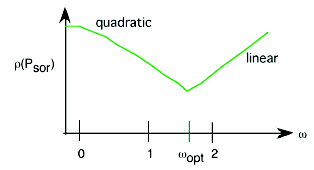
\includegraphics[height=2.25in]{../figs/SOR-omega}
\end{center}
\end{figure}

%--------------------------------------------------------------------
\subsection*{Number of Iterations?}

How many iterations does it take to reduce error by a factor of $\epsilon$? 
%For an idealized problem with $n$ unknowns and some constant $C_J$, we can say:
%%
%\begin{align}
%\rho(\ve{P}_J) &= 1 - C_J \frac{1}{n^2} + \dots \nonumber \\
%%
%\rho(\ve{P}_{GS}) &= 1 - 2 C_J \frac{1}{n^2} + \dots \nonumber \\
%%
%\rho(\ve{P}_{SOR}, \omega_{opt}) &= 1 - 2\sqrt{2 C_J} \frac{1}{n^2} + \dots \nonumber
%\end{align}
%%
%Then
%
\begin{align}
|| \vec{e}^{(k)} || &\leq \epsilon \: || \vec{e}^{(0)} || \nonumber \\
%
|| \vec{e}^{(k)} || &\leq \rho(\ve{P})^k || \vec{e}^{(0)} || \nonumber \\
%
\rho(\ve{P})^k &\approx \epsilon 
\qquad \text{take the log of both sides}\nonumber \\
%
k \log(\rho(\ve{P})) &\approx \log(\epsilon)\nonumber \\
%
k &\approx \frac{\log(\epsilon)}{\log(\rho(\ve{P}))} \nonumber
\end{align}

%--------------------------------------------------------------------
\subsection*{Preconditioning}
Condition number information is derived from Trefethen and Bau \cite{Trefethen1997}. Conditioning is one way to express the perturbation behavior of the mathematical problem. 

A \emph{well-conditioned} problem is one in which all small perturbations of $x$ lead to only small changes in $f(x)$. Why might this be desirable?

An \emph{ill-conditioned} problem is one in which some small perturbation of $x$ leads to a large change in $f(x)$. Why might this be \textit{undesirable}?

The condition number is a quantity used to express how well-conditioned a matrix or problem is. A small condition number corresponds to a well-conditioned problem, and vice versa. 

The \textbf{condition number} of a matrix $\mathbf{A}$ is defined as
\[\kappa(\mathbf{A}) = ||\mathbf{A}|| \text{ }||\mathbf{A}^{-1}|| \:.
\]
%
If the 2-norm is used, then $||\mathbf{A}||_{2} = \sigma_{1}$, $||\mathbf{A}^{-1}||_{2} = 1 / \sigma_{m}$, and $\kappa_{2}(\mathbf{A}) = \sigma_{1} / \sigma_{m}$; $\sigma_{m}$ is the $m$th singular value of $\ve{A}$. If $\mathbf{A}$ is singular, its condition number is infinity. 

The base-b logarithm of $\kappa$ is an estimate of how many base-b digits are lost in solving a linear system with that matrix. In other words, it estimates worst-case loss of precision. A system is said to be singular if the condition number is infinite, and ill-conditioned if it is too large, where ``too large" means roughly $\log(\kappa) >\sim$ the precision of matrix entries. %http://mathworld.wolfram.com/ConditionNumber.html

The general idea of \textbf{preconditioning} is to transform the system of interest into another equivalent system that has more favorable properties, for example one with a smaller condition number. 

A \textbf{preconditioner} is a matrix that induces such a transformation by improving the spectral properties of the problem being solved. 

Let $\ve{G}$ be a non-singular preconditioner, then \cite{Benzi2002} $\ve{A}\vec{x}=\vec{b}$ can be transformed as 
\[ \ve{G}^{-1}\ve{A}x = \ve{G}^{-1}b \:.\] 

Strictly speaking, Jacobi is ``preconditioned Richardson iteration", with $\ve{G} = \ve{D}$.
%in the following ways \cite{Benzi2002}: 
%%
%\begin{alignat}{3}
%  \ve{G}^{-1}\ve{A}x &= \ve{G}^{-1}b  &  &\text{left preconditioning,} \\
%  \ve{AG}^{-1}y &= b, \qquad  &x = \ve{G}^{-1}y \qquad &\text{right preconditioning, and } \\
%  \ve{G}_{1}^{-1}\ve{AG}_{2}^{-1}y &= \ve{G}_{1}^{-1}b, \qquad \ve{G} = \ve{G}_{1}\ve{G}_{2}, \qquad  &x = \ve{G}_{2}^{-1}y  \qquad &\text{split preconditioning.} 
%\end{alignat}
%
%If $\ve{A}$ and/or $\ve{G}$ are non-normal then each of the preconditioning constructs will likely give different behavior, though they will converge to the same answer because the matrices are similar and therefore have the same eigenvalues  \cite{Benzi2002}. Right preconditioning leaves the right hand side of the equation unaffected and does not change the norm of the residual, which is used for convergence testing in most iterative methods. Right preconditioning is usually preferred over left preconditioning for iterative solvers for this reason \cite{Knoll2004}. A right preconditioner was implemented in this work, and the remaining discussion will be presented in right preconditioner format. 

%The matrix $\ve{A}\ve{G}^{-1}$ is not formed in practice. The preconditioner can be applied by using some method to solve $\ve{G}y=c \to y \approx \ve{G}^{-1}c$, or by otherwise implementing the action of $\ve{G}^{-1}$ without ever explicitly forming and inverting $\ve{G}$. There are two extremes between which all other preconditioners lie: $\ve{G} = \ve{A}$, in which case the solution can be found directly, and $\ve{G} = \ve{I}$, which will have no effect \cite{Benzi2002}, \cite{Trefethen1997}. 

Functionally, a good preconditioner should make the system easier to solve and result in faster convergence. It should also be cheap to construct and apply. %These tend to be competing goals in that the easier a preconditioner is to construct and apply the less it typically does to improve convergence. A preconditioner is considered good if $\ve{A}\ve{G}^{-1}$ is not too far from normal and its eigenvalues are clustered \cite{Trefethen1997}. 

There are many different types of preconditioners, but they can be put into two general categories: \textbf{matrix-based} and \textbf{physics-based}.

\underline{Matrix-based} preconditioners rely entirely on the structure of the matrix $\ve{A}$ regardless of the physics of the problem. That is, these methods do not change when the underlying problem changes. This can be a very useful property because matrix-based methods are then broadly applicable and do not require any understanding of the physical problem \cite{Trefethen1997}. %Extrapolation methods and incomplete factorizations are examples of matrix-based preconditioners \cite{Trefethen1997}.

\underline{Physics-based} preconditioning uses knowledge about the physics of the problem in question to guide the creation of the preconditioner. This means that some methods only work with certain kinds of problems, and that the preconditioners may have to be tailored or adapted for different applications. However, such methods take advantage of knowing something about the problem and can be more effective than matrix-based methods for the range of problems for which they are intended \cite{Trefethen1997}. %Rebalance and synthetic acceleration are examples of physics-based preconditioners \cite{Trefethen1997}.


%--------------------------------------------------------------------
\clearpage
\subsection*{Examples}

Let's look at 
%
\begin{equation}
\begin{pmatrix}
  4  &  3 & 0 \\
  3  &  4 & -1 \\
  0  & -1 & 4
\end{pmatrix}
%
\begin{pmatrix} x_1 \\ x_2 \\ x_3 \end{pmatrix} 
%
= \begin{pmatrix} 24 \\ 30 \\ -24 \end{pmatrix} \nonumber
\end{equation}
%
with Jacobi, GS, and SOR. In each case we'll start with $\vec{x}^{(0)} = [1, 1, 1]^T$. The exact solution is $[3, 4, -5]^T$. 

%-------------------------------------------------------------------
\textbf{Jacobi:} for $i = 1, \dots, n$:
\[ x^{(k+1)}_i = \frac{1}{a_{ii}}(b_i - \sum_{j=1}^{i-1} a_{ij} x_j^{(k)} - \sum_{j=i+1}^{n} a_{ij} x_j^{(k)}) \:.\]
%
\begin{align*}
x_1^{(k+1)} &= \frac{1}{a_{11}}(b_{1} - a_{12} x_2^{(k)} - a_{13} x_3^{(k)}) = \frac{1}{4}(24 - 3 x_2^{(k)} - 0 x_3^{(k)}) = 6 - \frac{3}{4}x_2^{(k)}  \\
%
\\
x_2^{(k+1)} &= \frac{1}{a_{22}}(b_2 - a_{21} x_1^{(k)} - a_{23} x_3^{(k)}) = \frac{1}{4}(30 - 3 x_1^{(k)} - (-1) x_3^{(k)})= \frac{30}{4} - \frac{3}{4}x_1^{(k)} + \frac{1}{4}x_3^{(k)} \\
%
\\
x_3^{(k+1)} &= \frac{1}{a_{33}}(b_3 - a_{31} x_1^{(k)} - a_{32} x_2^{(k)}) = \frac{1}{4}(-24 - 0 x_1^{(k)} - (-1) x_2^{(k)}) = -6 + \frac{1}{4}x_2^{(k)}
\end{align*}

%-------------------------------------------------------------------
\textbf{GS:} for $i = 1, \dots, n$:
\[ x^{(k+1)}_i = \frac{1}{a_{ii}}(b_i - \sum_{j=1}^{i-1} a_{ij} x_j^{(k+1)} - \sum_{j=i+1}^{n} a_{ij} x_j^{(k)}) \:.\]
%
\begin{align*}
x_1^{(k+1)} &= \frac{1}{a_{11}}(b_{1} - a_{12} x_2^{(k)} - a_{13} x_3^{(k)}) = \frac{1}{4}(24 - 3 x_2^{(k)} - 0 x_3^{(k)}) = 6 - \frac{3}{4}x_2^{(k)}  \\
%
\\
x_2^{(k+1)} &= \frac{1}{a_{22}}(b_2 - a_{21} x_1^{(k+1)} - a_{23} x_3^{(k)}) = \frac{1}{4}(30 - 3 x_1^{(k+1)} - (-1) x_3^{(k)}) 
= \frac{30}{4} - \frac{3}{4}x_1^{(k+1)} + \frac{1}{4}x_3^{(k)}\\
%
\\
x_3^{(k+1)} &= \frac{1}{a_{33}}(b_3 - a_{31} x_1^{(k+1)} - a_{32} x_2^{(k+1)}) = \frac{1}{4}(-24 - 0 x_1^{(k+1)} - (-1) x_2^{(k+1)}) = -6 + \frac{1}{4}x_2^{(k+1)}
\end{align*}

%-------------------------------------------------------------------
\textbf{SOR:} for $i = 1, \dots, n$:
\[ x^{(k+1)}_i = (1-\omega)x_i^{(k)} + \frac{\omega}{a_{ii}}(b_i - \sum_{j=1}^{i-1} a_{ij} x_j^{(k+1)} - \sum_{j=i+1}^{n} a_{ij} x_j^{(k)}) \:.\]
%
Let $\omega = 1.25 = 5/4$
%
\begin{align*}
x_1^{(k+1)} &= (1-\omega)x_1^{(k)} + \frac{\omega}{a_{11}}(b_{1} - a_{12} x_2^{(k)} - a_{13} x_3^{(k)}) = (1-\frac{5}{4})x_1^{(k)} + \frac{\frac{5}{4}}{4}(24 - 3 x_2^{(k)} - 0 x_3^{(k)}) \\
&= \frac{15}{2} - \frac{1}{4}x_1^{(k)} - \frac{15}{16}x_2^{(k)}\\
%
\\
x_2^{(k+1)} &= (1-\omega)x_2^{(k)} + \frac{\omega}{a_{22}}(b_2 - a_{21} x_1^{(k+1)} - a_{23} x_3^{(k)})
= (1-\frac{5}{4})x_2^{(k)} + \frac{\frac{5}{4}}{4}(30 - 3 x_1^{(k+1)} - (-1) x_3^{(k)}) \\
&= \frac{150}{16} - \frac{15}{16}x_1^{(k+1)} - \frac{1}{4}x_2^{(k)} + \frac{5}{16}x_3^{(k)} \\
%
\\
x_3^{(k+1)} &= (1-\omega)x_3^{(k)} + \frac{\omega}{a_{33}}(b_3 - a_{31} x_1^{(k+1)} - a_{32} x_2^{(k+1)}) = (1-\frac{5}{4})x_3^{(k)} + \frac{\frac{5}{4}}{4}(-24 - 0 x_1^{(k+1)} - (-1) x_2^{(k+1)}) \\
&= -\frac{15}{2} + \frac{5}{16}x_2^{(k+1)} - \frac{1}{4}x_3^{(k)}
\end{align*}

\begin{table}[h]
  \caption{Jacobi}
  \centering
\begin{tabular}{| c | c | c | c | c | c | c |}
\hline
k & 0 & 1 & 2 & 3 & 4 & $|$error$|$ \\ \hline
$x_1$ & 1 & 5.25  & 0.75  & 4.40625  & 1.59375  & 1.40625\\ \hline 
$x_2$ & 1 & 7.0   & 2.125 & 5.875    & 2.82813  & 1.17188 \\ \hline 
$x_3$ & 1 & -5.75 & -4.25 & -5.46875 & -4.53125 & 0.46875 \\ \hline 
\end{tabular}

\caption{Gauss Seidel}
\begin{tabular}{| c | c | c | c | c | c | c |}
\hline
k & 0 & 1 & 2 & 3 & 4 & $|$error$|$ \\ \hline
$x_1$ & 1 & 5.25 & 3.140625 & 3.087891 & 3.05493 & 0.05493\\ \hline 
$x_2$ & 1 & 3.8125 & 3.8828125 & 3.92676 & 3.95422 & 0.04578 \\ \hline 
$x_3$ & 1 & -5.046875 & -5.0292969 & -5.01831 & -5.01144 & 0.01144\\ \hline 
\end{tabular}

\caption{SOR}
\begin{tabular}{| c | c | c | c | c | c | c |}
\hline
k & 0 & 1 & 2 & 3 & 4 & $|$error$|$ \\ \hline
$x_1$ & 1 & 6.3125 & 2.6223 & 3.1333 & 2.95705 & 0.04295 \\ \hline 
$x_2$ & 1 & 3.51953 & 3.95853 & 4.01026 & 4.00748 & 0.00748 \\ \hline 
$x_3$ & 1 & -6.65015 & -4.60042 & -5.096686 & -4.97349 & 0.02651 \\ \hline 
\end{tabular}
\end{table}


%--------------------------------------------------------------------
%--------------------------------------------------------------------
\bibliographystyle{plain}
\bibliography{13-14-iterative-solvers} 

\end{document}
